% !TEX encoding = UTF-8 Unicode
% !TEX root = SystemTemplate.tex

\documentclass{book}
% !TEX root = SystemTemplate.tex

\usepackage[width=6.5in, height=9.2in, top=1.0in, papersize={8.5in,11in}]{geometry}
\usepackage[pdftex]{graphicx}
%\usepackage{draftwatermark}
\usepackage{amsmath}
\usepackage{amsthm}
\usepackage{amssymb}
%\usepackage{txfonts}
\usepackage{textcomp}
%\usepackage{amsthm}

\usepackage[all]{xy}
\usepackage{fancyhdr}
\pagestyle{fancy}
\usepackage{hyperref}
\usepackage{verbatim}
\usepackage{algorithm}
\usepackage{algorithmic}
\usepackage{array}
\usepackage{color}
\usepackage{listings}
\lstset{language=c,frame=ltrb,framesep=5pt,basicstyle=\normalsize,
 keywordstyle=\ttfamily\color{DarkRed},
identifierstyle=\ttfamily\color{DarkBlue}\bfseries,
commentstyle=\color{OliveGreen},
stringstyle=\ttfamily,
showstringspaces=false,tabsize = 3}
\usepackage{calc}
\usepackage{doxygen}
\usepackage[utf8]{inputenc}
\usepackage{makeidx}
\usepackage{multicol}
\usepackage{multirow}
\usepackage[table]{xcolor}

\definecolor{color02}{rgb}{0.18,0.35,0.59}
\definecolor{color03}{rgb}{0.44,0.59,0.82}
\definecolor{color06}{rgb}{0.35,0.35,0.35}


\newtheorem{summary}{Summary:}
\newtheorem{example}{Example:}


\definecolor{OliveGreen}{cmyk}{0.64,0,0.95,0.40}
\definecolor{DarkBlue}{cmyk}{0.76,0.76,0,0.20}
\definecolor{DarkRed}{cmyk}{0,1,1,0.45}


\def      \RR             {{\mathbb R}} 
\def      \DS            {\displaystyle} 

\setlength{\oddsidemargin}{0mm} 
\setlength{\evensidemargin}{0mm} 

%\SetWatermarkLightness{0.975}
%\SetWatermarkScale{6}
%\SetWatermarkText{\includegraphics{test.png}}

\pagestyle{fancy}
\renewcommand{\chaptermark}[1]{\markboth{#1}{}}
\renewcommand{\sectionmark}[1]{\markright{\thesection\ #1}}
\fancyhf{}
\fancyhead[LE,RO]{\bfseries\thepage}
\fancyhead[LO]{\bfseries\rightmark}
\fancyhead[RE]{\bfseries\leftmark}
\fancyfoot[LE,RO]{Confidential and Proprietary}
%\renewcommand{\headrulewidth}{0.5pt}
%\renewcommand{\footrulewidth}{0pt}
%\addtolength{\headheight}{0.5pt}
%\setlength{\footskip}{0mm}
%\renewcommand{\footruleskip}{0pt}


\definecolor{MSBlue}{rgb}{.204,.353,.541}
\definecolor{MSLightBlue}{rgb}{.31,.506,.741}
\definecolor{MSBlue1}{rgb}{0.18,0.35,0.59}
\definecolor{MSBlue2}{rgb}{0.44,0.59,0.82}
\definecolor{MSBlue3}{rgb}{0.35,0.35,0.35}


\usepackage{titlesec}
\titleformat{\chapter}[display]
{\normalfont\bfseries\color{MSBlue1}}    %\normalfont\bfseries\filcenter}
{\LARGE\thechapter}
{1ex}
{\titlerule[2pt]
\vspace{2ex}%
\LARGE}
[\vspace{1ex}%
{\titlerule[2pt]}]

\definecolor{MSBlue}{rgb}{.204,.353,.541}
\definecolor{MSLightBlue}{rgb}{.31,.506,.741}
\definecolor{MSBlue1}{rgb}{0.18,0.35,0.59}
\definecolor{MSBlue2}{rgb}{0.44,0.59,0.82}
\definecolor{MSBlue3}{rgb}{0.35,0.35,0.35}

%\titleformat*{\section}{\Large\bfseries\sffamily\color{MSBlue}}
%\titleformat*{\subsection}{\large\bfseries\sffamily\color{MSLightBlue}}
%\titleformat*{\section}{\Large\bfseries\color{MSBlue1}}
%\titleformat*{\subsection}{\large\bfseries\color{MSBlue2}}

\titleformat*{\section}{\Large\bfseries\color{MSBlue}}
\titleformat*{\subsection}{\large\bfseries\color{MSLightBlue}}
\titleformat*{\subsubsection}{\large\bfseries\color{MSBlue3}}
\setcounter{secnumdepth}{3}
\renewcommand{\thesubsubsection}{\thesubsection.\alph{subsubsection}}

 % This sets the format.

% Add your title page contents here 
\title{{\color{MSBlue1} \rule{\linewidth}{0.5mm}}\\[2mm] {\huge \bfseries \color{MSBlue1} C++ Automated Test Suite }\\[-1mm] {\color{MSBlue1}\rule{\linewidth}{0.5mm}} \\  \vfill
{\LARGE \bfseries \color{MSBlue2} Software Engineering Documentation }\\  \vfill 
{\color{MSBlue1} Intolerable Optimists } }
\author{\color{MSBlue1}  Charles Parsons \and \color{MSBlue1} Christopher Smith \and  \color{MSBlue1} Jarod Hogan }
\date{\color{MSBlue1} \today}


\begin{document}
\frontmatter
\maketitle


\tableofcontents
\listoffigures
\listoftables
\listofalgorithms


% !TEX root = SystemTemplate.tex

\chapter{Mission}

\textbf{Our mission:}
\\
\\To explore strange new worlds...
\\To seek out new life and new civilizations...
\\To boldly go where no man has gone before...
\\
\\Wait...
\\
\\No...
\\
\\ \textbf{We meant:}
\\
\\To design and implement an automatic testing system that will completely and effectively meet the grading needs of amazing Computer Science professors everywhere, in order to enable them to live happier, less stressful, more fulfilling, richer lives with more time for The Daily Show.  % add mission statement to mission.tex
% !TEX root = SystemTemplate.tex

\chapter{Document Preparation and Updates}

Current Version [1.0.0]
\vspace*{5mm}

{\color{MSBlue3}
\noindent
\textit{Prepared By:}\\
\textit{Erik Hattervig}\\
\textit{Andrew Koc}\\
\textit{Jonathan Tomes}
}

\vfill
\noindent
{\color{color02} \textit{\textbf{Revision History}}}\\
\begin{tabular}{|>{\raggedright}p{1.5cm}|>{\raggedright}p{3cm}|>{\raggedright}p{1.5cm}|>{\raggedright}p{9cm}|}
\hline
\textit{\textbf{Date}} &  \textit{\textbf{Author}} & \textit{\textbf{Version}} & \textit{\textbf{Comments}}\tabularnewline
\hline
 \textit{\textbf{2/2/12}} & \textit{Team Member \#3} & \textit{1.0.0} & \textit{Initial version}\tabularnewline
\hline
\textit{\textbf{3/4/12}} & \textit{Team Member \#3} & \textit{1.1.0} & \textit{Edited version}\tabularnewline
\hline
 &  &  & \tabularnewline
 \hline
 &  &  & \tabularnewline
\hline
 &  &  & \tabularnewline
\hline
 &  &  & \tabularnewline
\hline
 &  &  & \tabularnewline
\hline
\end{tabular}
\vfill



 
\mainmatter

%%  Add to the following chapters

% !TEX root = SystemTemplate.tex

\chapter{Overview and concept of operations}

This system is for professors to test their students’ programs against test data contained in text files. The results of these tests will then be written to a text file for th user to evaluate the tested programs performance.

Title: Dr. Logar’s User Story As a professor I want to have a program compile, run, test, and evaluate the tests run on a program submitted to me by my students so that I no longer have to run each test case individually and evaluate them by hand.
The progam should compile and run a program against all test cases contained in files ending in ”.tst” within the current directory or within a subdirectory. In addition, it will evaluate the passes and fails of the program and log this in a text document for user review.
Titile: Revisions to make life  easier. It is also desired that this test suite runs all test files contained in a test directory against each program submitted by a student. Each student will have their own directory where the result file should be stored. 
Title: Automatic tests. As I am quite I would like to have the test suite generate its own tests so that I don't have to. It will store these tests in the tests subdirectory and generate the answer file for each test. 





\section{Scope}
The purpose of this project is to create a program that will run another program against test documents and output the 
results into another file forthe user. The program is specifically geared toward computer science professors for their use in 
grading student programs. This program will compile and run the submitted program imputting the test data. The results, which are saved to a text document, are evaluated and and percentage of pass/fail is also computed and saved in the
document.


\section{Purpose}
This system is designed in order to make it easier for professors to grade their students programs. The test files need only be 
in the same directory (or within a subdirectory) as the program to be compiled and run. Also, the output is to be detailed 
enough so that the user knows exactly which test cases passed and which failed.


\subsection{Program Compiler}
Though rather simple to code this is a mojor component because it depends on which system the program is running as to
how the program is compiled. This program is made to run using the gcc command.

\subsection{Test File Location}
Also a simple but necessary component to our system. The program is going to run every file ending in ".tst" within the same
directory as the progam itself. Therefore, searching the current working directory as well as every subdirectory is very 
important to ensure every test case is run.

\subsection{Test Case Evaluation}
Here is the most critical part of the program. This is where the tests are read in by our program and the results evaluated. 
Once evaluated the results are stored in a text file for the user to review. We will test various different possbile directory orderings as well as the ability to run against varying types of test cases.

\section{Systems Goals}
The goals of our system is to successfully compile and run a program with the test files in the directory. Then to output the result of the tests in a text file. It is also our goal to generate our own test cases for the user and generate cooresponding answer files.

\section{System Overview and Diagram}
The system flow is pretty simple. The program will walk through directories searching for test cases to run student programs on. With this resent update we have a specific file directory we expect. This program will be placed in the root directory. In this root directory will be a subdirectory for each student as well as a tests subdirectory, which will naturally store the tests. There will also be a golden.cpp in the root directory. This program, if prompted, will generate test cases and store them in the tests subdirectory and will use the golden.cpp to generate anwer files which will be placed in the root directory. Afterwards, the program will walk through the students directories and run their program against all the tests and give them a grade. 

\begin{figure}[tbh]
\begin{center}
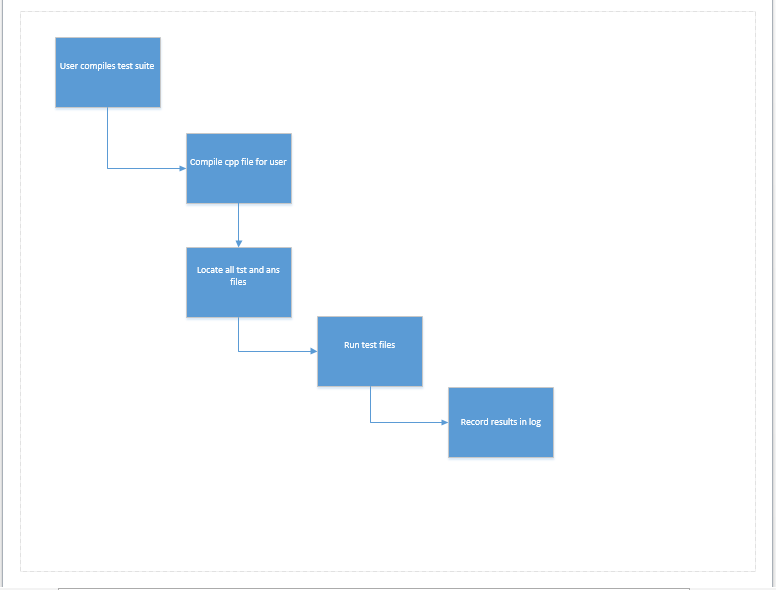
\includegraphics[width=0.75\textwidth]{./Diagran}
\end{center}
\caption{A sample figure .... System Diagram \label{systemdiagram}}
\end{figure}

\section{Technologies Overview}
There was no need for wide range of technologies in this specfic program. However, we have made extensive use of some software to enable us to be productive. Firstly we have used GitHub for version control. We used Trello to keep everybody on track and give an easy place to comunicate job assignments. Finally, but most importantly we used the Linux operating system on the Fujitsu tablets to do all our programing.   
\begin{table}[tbh]
\begin{center}
\begin{tabular}{|r|l|}
  \hline
  7C0 & hexadecimal \\
  3700 & octal \\ \cline{2-2}
  11111000000 & binary \\
  \hline \hline
  1984 & decimal \\
  \hline
\end{tabular}
\caption{A sample Table ... some numbers. \label{somenumbers}}
\end{center}
\end{table}


% !TEX root = SystemTemplate.tex


\chapter{Project Overview}
This section provides some housekeeping type of information with regard to the 
team, project, etc. 



\section{Team Members and Roles}
The team consists of Erik Hattervig, Andrew Koc, and Jonathon Tomes. Erik Hattervig is the Product Owner, Andrew Koc is the Technical Lead, and Jonathon Tomes is the Scrum Master. Erik is responsible for understanding the overall expectations of the product and communication with the customer about specific details regarding the operation and design of the product. Andrew is responsible for designing the technical aspects of the code. Jonathon is responsible for managing meetings and communication between team members and making sure the project is on schedule.


\section{Project  Management Approach}
%This section will provide an explanation of the basic approach to managing the 
%project.  Typically, this would detail how the project will be managed through 
%a given Agile methodology.  The sprint length (i.e. 2 weeks) and product backlog 
%ownership and location (ex. Trello) are examples of what will be discussed.  An 
%overview of the system used to track sprint tasks, bug or trouble tickets, and 
%user stories would be warranted.

	The sprint length for this project was 2 weeks. We began with a meeting to
decide the user needs and split the program accordingly. Each of us would code
different parts of the program and then we would all test and re-code as needed.

	The code was stored, backed up, and shared through git hub. The back log and ownership 
was tracked through Trello. The user stories were condensed and placed on Trello to help 
design break points to split up the program between team members. 

\section{Phase  Overview}
%If the system will be implemented in phases, describe those phases/sub-phases (design, 
%implementation, testing, delivery) and the various milestones in this section. 
 %This section should also contain a correlation between the phases of development 
%and the associated versioning of the system, i.e. major version, minor version, 
%revision. 

The first phase of this Testing program was just to begin working on the program.
The main purpose was to get to receive a root directory, find a .cpp file
in the root. It would then write a log file that starting with a time stamp to
be used later to record the results of tests.
	
	After that it would a crawl through the sub directories recursively
starting at the root, looking for .tst files that would be test cases for 
the program. Along with these would be .ans files that would allow us to
compare the program output and see wich test cases failed. 
	
	It would then out put the results of each test to a log file. With a final
log write that writes the percentage of passed and failed tests.

\section{Terminology and Acronyms}
%Provide a list of terms used in the document that warrant definition.  Consider 
%industry or domain specific terms and acronyms as well as system specific.
none. 

% !TEX root = SystemTemplate.tex
\chapter{User Stories, Backlog and Requirements}
\section{Overview}

This document contains a summary of what we, The Software Engineering Adventure Line, did during the development of our Program Tester program. The Program Tester is designed to aid professors and TAs in grading student programs by allowing users to write test cases to be performed on the student programs and have a summary of how well the student programs did generated.


%The overview should take the form of an executive summary.  Give the reader a feel 
%for the purpose of the document, what is contained in the document, and an idea 
%of the purpose for the system or product. 

% The userstories 
%are provided by the stakeholders.  You will create he backlogs and the requirements, and document here.  
%This chapter should contain 
%details about each of the requirements and how the requirements are or will be 
%satisfied in the design and implementation of the system.

%Below:   list, describe, and define the requirements in this chapter.  
%There could be any number of sub-sections to help provide the necessary level of 
%detail. 





\subsection{Scope}
This document covers our basic user stories and requirements for this program.

% What scope does this document cover?  This document would contain stakeholder information, 
% initial user stories, requirements, proof of concept results, and various research 
% task results. 



\subsection{Purpose of the System}
This Program is meant to be used in an academic setting to grade student programs. 
This will help educators streamline their grading process by taking out the need to 
compile and test each program individually.

% What is the purpose of the system or product? 


\section{ Stakeholder Information}
This products main stakeholders are professors and TA in education.
The program assists them in grading programs that they receive from students. 
This task can be done manually so this program is not critical to their needs but is a 
great convenience as it saves time during the grading process.

% This section would provide the basic description of all of the stakeholders for 
% the project.  Who has an interest in the successful and/or unsuccessful completion 
% of this project? 


\subsection{Customer or End User (Product Owner)}
Erik Hattervig is the Product Owner of this project. He is in charge of understanding the requirements set forth by our
customer, Dr. A. Logar, managing the product backlog, keeping the rest of the team up to date on what
needs to be done in an overall sence, and writing a portion of the code that is required.

% Who?  What role will they play in the project?  Will this person or group manage 
% and prioritize the product backlog?  Who will they interact with on the team to 
% drive product backlog priorities if not done directly? 

\subsection{Management or Instructor (Scrum Master)}
Jonathan Tomes is the Scrum of this project. He is in charge of managing the schedules of other team members
and keeping track of the sprints of the project.

% Who?  What role will they play in the project?  Will the Scrum Master drive the 
% Sprint Meetings? 


\subsection{Investors}
Investors in this project include Dr Logar, who has set the requirements of the project and the specifications for it.

% Are there any?  Who?  What role will they play? 


\subsection{Developers --Testers}
All three of the members of this team will be testing the program to make sure it works as intened.

%Who?  Is there a defined project manager, developer, tester, designer, architect, 
%etc.? 


\section{Business Need}
This program speeds up the process of grading programs for professors in academia, and save unnecessary repetitive work from needing to be done manually. 

%Use this section to define what business need exist and how this software will 
%meet and/or exceed that business need.   

\section{Requirements and Design Constraints}
This program has been designed to be used on a Linux System and does not requires very many system resources to be run. The program will not run on a Windows system in its current state.
%Use this section to discuss what requirements exist that deal with meeting the 
%business need.  These requirements might equate to design constraints which can 
%take the form of system, network, and/or user constraints.  Examples:  Windows 
%Server only, iOS only, slow network constraints, or no offline, local storage capabilities. 


%\subsection{System  Requirements}
%What are they?  How will they impact the potential design?  Are there alternatives? 


%\subsection{Network Requirements}
%What are they? 


\subsection{Development Environment Requirements}
The program has been developed for use on a Linux System.
%What are they?  Is the system supposed to be cross-platform? 


\subsection{Project  Management Methodology}
%The stakeholders might restrict how the project implementation will be managed. 
% There may be constraints on when design meetings will take place.  There might 
%be restrictions on how often progress reports need to be provided and to whom. 
 
\begin{itemize}
\item We are using Trello to keep track of the backlogs and sprint status.%What system will be used to keep track of the backlogs and sprint status?
\item All Parties will have access to the Sprint and Product Backlogs via Trello.%Will all parties have access to the Sprint and Product Backlogs?
\item This project will encompass on sprint.%How many Sprints will encompass this particular project?
\item The Sprint Cycles are one week long.%How long are the Sprint Cycles?
\item We are using GitHub for our source control and there are currently no restrictions for team members on it.%Are there restrictions on source control? 
\end{itemize}

\section{User Stories}
%This section can really be seen as the guts of the document.  This section should 
%be the result of discussions with the stakeholders with regard to the actual functional 
%requirements of the software.  It is the user stories that will be used in the 
%work breakdown structure to build tasks to fill the product backlog for implementation 
%through the sprints.

%This section should contain sub-sections to define and potentially provide a breakdown 
%of larger user stories into smaller user stories. 



\subsection{User Story \#1}
As a user I want the program to read in the .tst files and test them on the program.

We want to read in .tst file and run them on the compiled program.

%\subsubsection{User Story \#1 Breakdown}
%Does the first user story need some division into smaller, consumable parts by 
%the reader?  This does not need to go to the level of actual task definition and 
%may not be required. 

\subsection{User Story \#2} 
As a user I want the program to compile the .cpp file.

We want to be able to compile the student's .cpp file that is in the root directory.


%\subsubsection{User Story \#2 Breakdown}
%User story \#2  .... 

\subsection{User Story \#3} 
As a user I want the program to store the percentage of pass and failed test cases in the .log file

\subsection{User Story \#4}
As a user I want the program to crawl through a directory looking for .tst files.
 We want to be able to crawl through all subdirectories looking for .tst files to test on.


%\subsubsection{User Story \#3 Breakdown}
%User story \#3  .... 


%\section{Research or Proof of Concept Results}
%This section is reserved for the discussion centered on any research that needed 
%to take place before full system design.  The research efforts may have led to 
%the need to actually provide a proof of concept for approval by the stakeholders. 
%The proof of concept might even go to the extent of a user interface design or 
%mockups. 


%\section{Supporting Material}


%This document might contain references or supporting material which should be documented 
%and discussed  either here if approprite or more often in the appendices at the end.  This material may have been provided by %the stakeholders  
%or it may be material garnered from research tasks.


% !TEX root = SystemTemplate.tex
\chapter{Design  and Implementation}

\section{Major Component \#1 }

\subsection{Technologies  Used}
Text editor used was Vim. Development was done on the Linux OS.

\subsection{Component  Overview}
Testing Suite for C++ programs.

\subsection{Phase Overview}
Initial phase for testing suite. Suite runs a single executable compiled from a *.cpp file against *.tst files.

\subsection{ Architecture  Diagram}
Compile a *.cpp file passed as a command line argument. Run that executable against all *.tst files within the
current directory and all of its sub-directories.


\subsection{Data Flow Diagram}
Input is redirected from the *.tst file and output is redirected to a *.out file. The *.out file is compared to the
corresponding *.ans file. The results are printed in a *.log file.


\subsection{Design Details}




\section{Major Component \#2 }

\subsection{Technologies  Used}


\subsection{Component  Overview}


\subsection{Phase Overview}


\subsection{ Architecture  Diagram}



\subsection{Data Flow Diagram}



\subsection{Design Details}



\section{Major Component \#3 }

\subsection{Technologies  Used}


\subsection{Component  Overview}


\subsection{Phase Overview}


\subsection{ Architecture  Diagram}


\subsection{Data Flow Diagram}



\subsection{Design Details}




% !TEX root = SystemTemplate.tex

\chapter{System  and Unit Testing}

\section{Overview}
Unit testing on individual source code functions occurred during the development process. The programmers utilized a {\it transparent-box} testing approach to ensure their functions performed correctly with expected, edge-case, and unexpected input.\\\\
A {\it black-box} approach was used to test the functional requirements of the system. See section 5.3 {\it (Test Setup and Execution)} for more information on system requirements testing.

\section{Dependencies}
Successful execution of this program depends on a correct class directory structure. See Figure ~\ref{directorylayout} for more information on this structure.


\section{Test Setup and Execution}
The following test matrix was constructed to ensure the functional requirements of the program. Each row in the table (See Table~\ref{SysReqtable}) represents a test case. Columns in the table represent functional requirements of the program. The results of each test are recorded with respect to each of the requirements.
\pagebreak
\begin{center}
\checkmark = Expected Results, x = Failing Results
\end{center}

\begin{table}[tbh]
\begin{center}
\begin{tabular}{| l | l | l | l |}


\hline
Test Case & Program Execution & Main Log File & Individual Log Files \\ \hline
   
    No student files and no test files & \multicolumn{1}{|c|}{\checkmark} & \multicolumn{1}{|c|}{\checkmark} & \multicolumn{1}{|c|}{\checkmark} \\ \hline
    
    No student files and test files & \multicolumn{1}{|c|}{\checkmark} & \multicolumn{1}{|c|}{\checkmark} & \multicolumn{1}{|c|}{\checkmark} \\ \hline
    
   Student files and critical tests only & \multicolumn{1}{|c|}{\checkmark} & \multicolumn{1}{|c|}{\checkmark} & \multicolumn{1}{|c|}{\checkmark} \\ \hline
   
   Student files and non critical tests only & \multicolumn{1}{|c|}{\checkmark} & \multicolumn{1}{|c|}{\checkmark} & \multicolumn{1}{|c|}{\checkmark} \\ \hline
   
   One critical test and many normal tests & \multicolumn{1}{|c|}{\checkmark} & \multicolumn{1}{|c|}{\checkmark} & \multicolumn{1}{|c|}{\checkmark} \\ \hline
   
   Many critical tests and many normal tests & \multicolumn{1}{|c|}{\checkmark} & \multicolumn{1}{|c|}{\checkmark} & \multicolumn{1}{|c|}{\checkmark} \\ \hline
   
   Floating point tests only & \multicolumn{1}{|c|}{\checkmark} & \multicolumn{1}{|c|}{\checkmark} & \multicolumn{1}{|c|}{\checkmark} \\ \hline
   
   Integer tests only & \multicolumn{1}{|c|}{\checkmark} & \multicolumn{1}{|c|}{\checkmark} & \multicolumn{1}{|c|}{\checkmark} \\ \hline
   
   Student c++ files $\neq$ student directory name & \multicolumn{1}{|c|}{\checkmark} & \multicolumn{1}{|c|}{\checkmark} & \multicolumn{1}{|c|}{\checkmark} \\ \hline
   
   Students failing critical tests & \multicolumn{1}{|c|}{\checkmark} & \multicolumn{1}{|c|}{\checkmark} & \multicolumn{1}{|c|}{\checkmark} \\ \hline
   
   Students passing all tests & \multicolumn{1}{|c|}{\checkmark} & \multicolumn{1}{|c|}{\checkmark} & \multicolumn{1}{|c|}{\checkmark} \\ \hline
   
   Students passing critical tests but not all normal tests & \multicolumn{1}{|c|}{\checkmark} & \multicolumn{1}{|c|}{\checkmark} & \multicolumn{1}{|c|}{\checkmark} \\ \hline
   
   Integer test file generation & \multicolumn{1}{|c|}{\checkmark} & \multicolumn{1}{|c|}{N/A} & \multicolumn{1}{|c|}{N/A} \\ \hline
   
   Floating point test file generation & \multicolumn{1}{|c|}{\checkmark} & \multicolumn{1}{|c|}{N/A} & \multicolumn{1}{|c|}{N/A} \\ \hline
   
   Generate test files with no "golden" .cpp file & \multicolumn{1}{|c|}{x} & \multicolumn{1}{|c|}{N/A} & \multicolumn{1}{|c|}{N/A} \\ \hline
  
  Test program multiple times without exiting & \multicolumn{1}{|c|}{\checkmark} & \multicolumn{1}{|c|}{\checkmark} & \multicolumn{1}{|c|}{\checkmark} \\ \hline
  
  Generate test files multiple times without exiting & \multicolumn{1}{|c|}{\checkmark} & \multicolumn{1}{|c|}{N/A} & \multicolumn{1}{|c|}{N/A} \\ \hline
  
  Generate test files and test the programs without exiting & \multicolumn{1}{|c|}{\checkmark} & \multicolumn{1}{|c|}{\checkmark} & \multicolumn{1}{|c|}{\checkmark} \\ \hline
  
  Improper numerical input for menu options & \multicolumn{1}{|c|}{\checkmark} & \multicolumn{1}{|c|}{\checkmark} & \multicolumn{1}{|c|}{\checkmark} \\ \hline
  
  Entering strings for numerical input & \multicolumn{1}{|c|}{x} & \multicolumn{1}{|c|}{x} & \multicolumn{1}{|c|}{x} \\ \hline

\end{tabular}
\caption{System Requirements Tests Table \label{SysReqtable}}
\end{center}
\end{table}






% !TEX root = SystemTemplate.tex
\chapter{Development Environment}
Since the program was to test files on a Linux enviornment, it was developed on a Linux enviornment.


\section{Development IDE and Tools}
No special Tools or IDE were used to develop this.  Since the code was so simple
each programmer just used what ever coding enviornment they wanted.  All
the code was tested on a Linux machine using the g++ compiler.  The debug tool
gdb was used to debug the code when necessary.

\section{Source  Control}
We used github for source control.  The repository can be found at this url: 

https://github.com/CsmithSD/IO_Soft_Eng
\section{Dependencies}
This program is dependent on the C++ Standard Library as well as the g++ compiler
on a Linux system.

\section{Build  Environment}
The execuatble is built by the g++ compiler.  You can either compile it manually, using the command:
\begin{lstlisting}
g++ -o tester ProgramTester.cpp
\end{lstlisting}
Or by using the following make file:

\begin{lstlisting}
# compiler
CC = g++

# compiler options
CFLAGS = -c -Wall

all: tester

tester: tester.o
	$(CC) -lm tester.o -o ProgramTester

tester.o: ProgramTester.cpp
	$(CC) $(CFLAGS) ProgramTester.cpp

clean:
	rm -rf *o tester
\end{lstlisting}


% !TEX root = SystemTemplate.tex

\chapter{Release -- Setup -- Deployment}
This section should contain any specific subsection regarding specifics in releasing, 
setup, and/or deployment of the system. 


\section{Deployment Information and Dependencies}
Are there dependencies that are not embedded into the system install? 



\section{Setup Information}
How is a setup/install built? 



\section{System  Versioning Information}
How is the system versioned? 

% !TEX root = SystemTemplate.tex

\chapter{User Documentation}

%This section should contain the basis for any end user documentation for the system. 
 %End user documentation would cover the basic steps for setup and use of the system. 
 %It is likely that the majority of this section would be present in its own document 
%to be delivered to the end user.  However, it is recommended the original is contained 
%and maintained in this document. 

%\newpage   %% 
%%  The user guide can be an external document which is included here if necessary ...
%%  a single source is the way to go.

\section{User Guide}

%The source for the user guide can go here.    You have some options for how to handle the user docs.  If you have some {\tt newpage} commands around the %guide then you can just print out those pages.   If a different formatting is required, then have the source in a separate file {\tt userguide.tex} and include %that file here.  That file can also be included into a driver (like the senior design template) which has the client specified formatting.  Again, this is a single %source approach.   

To use this testing program:
  
 1) make sure that you are in the directory where out program is installed.
 
 2) run the program with on the command line: tester (directory where cpp file and test files are present)
 
 The directory should be the full file path to the proper directory.
 
 Do not put parenthesis around the directory path.
 
 3) the tester program will write a log file to the directory where the cpp file is located.
 
This program is ment to be used with a Linux system.

%% \newpage  %%  if needed ...
\section{Installation Guide}
Insure that ProgramTester.cpp and makefile are in the same
 directory and just type "make" on the command line to install the program
 
 Alternatively you may just compile on the command line with:
 
 g++ ProgramTester.cpp -o tester
  
 Both of these require that you have g++ installed on your system.
 The program is meant to be used on a Linux system.

%% \newpage  %%  if needed ...
\section{Programmer Manual}


% !TEX root = SystemTemplate.tex

\chapter{Source Code File Index}
\section{Class List}
Here are the classes, structs, unions and interfaces with brief descriptions\-:\begin{DoxyCompactList}
\item\contentsline{section}{\hyperlink{class_poly}{Poly} }{\pageref{class_poly}}{}
\end{DoxyCompactList}

\chapter{Function Documentation}
\hypertarget{grade_8cpp}{\section{grade.\-cpp File Reference}
\label{grade_8cpp}\index{grade.\-cpp@{grade.\-cpp}}
}


Grade.\-cpp is designed to test computer programs against predefined test cases and answer files. Test cases contain output that may be provided to the program and answer files contain a correct solution. Test files may also be generated by the program. Generation is done based on user input to define the number of test files, file size, numeric range of entries, entry type (int or float), and an output file name.  


{\ttfamily \#include $<$fstream$>$}\\*
{\ttfamily \#include $<$cstdlib$>$}\\*
{\ttfamily \#include $<$iostream$>$}\\*
{\ttfamily \#include $<$string$>$}\\*
{\ttfamily \#include $<$dirent.\-h$>$}\\*
{\ttfamily \#include $<$cstring$>$}\\*
{\ttfamily \#include $<$vector$>$}\\*
{\ttfamily \#include $<$cmath$>$}\\*
{\ttfamily \#include $<$limits.\-h$>$}\\*
{\ttfamily \#include $<$iomanip$>$}\\*
{\ttfamily \#include $<$stdio.\-h$>$}\\*
{\ttfamily \#include $<$stdlib.\-h$>$}\\*
{\ttfamily \#include $<$time.\-h$>$}\\*
\subsection*{Functions}
\begin{DoxyCompactItemize}
\item 
void \hyperlink{grade_8cpp_aeb998e49bfc9ae3f7f872be6058a1f6b}{grade} (vector$<$ string $>$ crit\-Test\-Cases, vector$<$ string $>$ test\-Cases, vector$<$ string $>$ student\-Dirs, ofstream \&L\-O\-G, string exe\-Time)
\begin{DoxyCompactList}\small\item\em Run all student programs against all test cases. \end{DoxyCompactList}\item 
double \hyperlink{grade_8cpp_a8f45df268564e139b1488d2e9c9421e6}{calc\-\_\-percentage} (int passes, int total)
\begin{DoxyCompactList}\small\item\em Returns a floating point percentage (passed/total) \end{DoxyCompactList}\item 
void \hyperlink{grade_8cpp_ae8b8dbe94e2054e652ac25f63e3c0e47}{directory\-Crawl} (bool type, string dir, string file, bool recursive, vector$<$ string $>$ \&names, bool crit\-F\-L\-A\-G)
\begin{DoxyCompactList}\small\item\em Recursively crawls through a file system to find files or directory names. \end{DoxyCompactList}\item 
bool \hyperlink{grade_8cpp_a28a8333701b8a2c206c7bc8cd22ceeab}{test} (const string \&program, string a\-\_\-file, string tst\-\_\-file)
\begin{DoxyCompactList}\small\item\em This function will run a tst file with the compiled cpp file and compare the outputs of redirected output to a .out file with a .ans file by running a diff command. \end{DoxyCompactList}\item 
int \hyperlink{grade_8cpp_a04aefa2a2a2da275eaed20e26d447077}{print\-\_\-menu} ()
\begin{DoxyCompactList}\small\item\em Prints menu to let user choose between running test cases or creating new ones. \end{DoxyCompactList}\item 
bool \hyperlink{grade_8cpp_a6aab18b1906df07fc2cabf1d14b55c57}{create\-\_\-test\-\_\-cases} ()
\item 
double \hyperlink{grade_8cpp_a967ec1355894a4e49829049fe03721e8}{generate\-\_\-random} (double min, double max, char type)
\begin{DoxyCompactList}\small\item\em Generates a random integer or floating point number on the closed interval \mbox{[}min,max\mbox{]}. \end{DoxyCompactList}\item 
string \hyperlink{grade_8cpp_aa0b2b0d911e5107dc1cb4a77f9e8ea4b}{i\-To\-A} (int i)
\begin{DoxyCompactList}\small\item\em Converts an integer value to a string to append. \end{DoxyCompactList}\item 
bool \hyperlink{grade_8cpp_a7b59bf9d0451b8b79a0b200e8afdda38}{create\-\_\-ans\-\_\-file} (string test\-\_\-file\-\_\-path, string golden)
\begin{DoxyCompactList}\small\item\em This function runs the golden cpp on the test file to create the .ans file. \end{DoxyCompactList}\item 
bool \hyperlink{grade_8cpp_aea0e94853a0364481437dd133bf9079b}{compile\-\_\-code} (string filename)
\begin{DoxyCompactList}\small\item\em This function compiles the source code \char`\"{}filename.\-cpp\char`\"{} into an executable called \char`\"{}filename\char`\"{}. \end{DoxyCompactList}\item 
\hypertarget{grade_8cpp_a08ba7742fcc85f89113b95b1b85d7a5f}{bool {\bfseries run\-\_\-code} (string, string)}\label{grade_8cpp_a08ba7742fcc85f89113b95b1b85d7a5f}

\item 
string \hyperlink{grade_8cpp_af69ac93f047cb13a2e8e52f535f8dfde}{remove\-Extension} (string file)
\begin{DoxyCompactList}\small\item\em Removes the extension from a file name. \end{DoxyCompactList}\item 
string \hyperlink{grade_8cpp_a530247c8731a46cb00aff5f496c527f3}{file\-Name\-From\-Path} (string file)
\begin{DoxyCompactList}\small\item\em Returns the file name from a path to a file. \end{DoxyCompactList}\item 
int \hyperlink{grade_8cpp_ae66f6b31b5ad750f1fe042a706a4e3d4}{main} ()
\begin{DoxyCompactList}\small\item\em Main entry point of program. \end{DoxyCompactList}\end{DoxyCompactItemize}
\subsection*{Variables}
\begin{DoxyCompactItemize}
\item 
\hypertarget{grade_8cpp_ab5dbdc67cf17008c89ec3af3f029fb89}{const bool {\bfseries F\-I\-L\-E\-S} = true}\label{grade_8cpp_ab5dbdc67cf17008c89ec3af3f029fb89}

\item 
\hypertarget{grade_8cpp_a4a0315ababb2858ca3b419ad5b83e4d5}{const bool {\bfseries D\-I\-R\-E\-C\-T\-O\-R\-I\-E\-S} = false}\label{grade_8cpp_a4a0315ababb2858ca3b419ad5b83e4d5}

\end{DoxyCompactItemize}


\subsection{Detailed Description}
Grade.\-cpp is designed to test computer programs against predefined test cases and answer files. Test cases contain output that may be provided to the program and answer files contain a correct solution. Test files may also be generated by the program. Generation is done based on user input to define the number of test files, file size, numeric range of entries, entry type (int or float), and an output file name. 

\subsection{Function Documentation}
\hypertarget{grade_8cpp_a8f45df268564e139b1488d2e9c9421e6}{\index{grade.\-cpp@{grade.\-cpp}!calc\-\_\-percentage@{calc\-\_\-percentage}}
\index{calc\-\_\-percentage@{calc\-\_\-percentage}!grade.cpp@{grade.\-cpp}}
\subsubsection[{calc\-\_\-percentage}]{\setlength{\rightskip}{0pt plus 5cm}double calc\-\_\-percentage (
\begin{DoxyParamCaption}
\item[{int}]{passes, }
\item[{int}]{total}
\end{DoxyParamCaption}
)}}\label{grade_8cpp_a8f45df268564e139b1488d2e9c9421e6}


Returns a floating point percentage (passed/total) 



 
\begin{DoxyParams}{Parameters}
{\em passes} & -\/ number of passed tests \\
\hline
{\em total} & -\/ Total number of tests \\
\hline
\end{DoxyParams}
\begin{DoxyReturn}{Returns}
Percentage (0-\/100) 
\end{DoxyReturn}
\hypertarget{grade_8cpp_aea0e94853a0364481437dd133bf9079b}{\index{grade.\-cpp@{grade.\-cpp}!compile\-\_\-code@{compile\-\_\-code}}
\index{compile\-\_\-code@{compile\-\_\-code}!grade.cpp@{grade.\-cpp}}
\subsubsection[{compile\-\_\-code}]{\setlength{\rightskip}{0pt plus 5cm}bool compile\-\_\-code (
\begin{DoxyParamCaption}
\item[{string}]{filename}
\end{DoxyParamCaption}
)}}\label{grade_8cpp_aea0e94853a0364481437dd133bf9079b}


This function compiles the source code \char`\"{}filename.\-cpp\char`\"{} into an executable called \char`\"{}filename\char`\"{}. 



 \begin{DoxyAuthor}{Author}
Daniel Nix 
\end{DoxyAuthor}

\begin{DoxyParams}{Parameters}
{\em filename} & -\/ the name of the .cpp file \\
\hline
\end{DoxyParams}
\begin{DoxyReturn}{Returns}
true -\/ When the code is successfully compiled 
\end{DoxyReturn}
\hypertarget{grade_8cpp_a7b59bf9d0451b8b79a0b200e8afdda38}{\index{grade.\-cpp@{grade.\-cpp}!create\-\_\-ans\-\_\-file@{create\-\_\-ans\-\_\-file}}
\index{create\-\_\-ans\-\_\-file@{create\-\_\-ans\-\_\-file}!grade.cpp@{grade.\-cpp}}
\subsubsection[{create\-\_\-ans\-\_\-file}]{\setlength{\rightskip}{0pt plus 5cm}bool create\-\_\-ans\-\_\-file (
\begin{DoxyParamCaption}
\item[{string}]{test\-\_\-file\-\_\-path, }
\item[{string}]{golden}
\end{DoxyParamCaption}
)}}\label{grade_8cpp_a7b59bf9d0451b8b79a0b200e8afdda38}


This function runs the golden cpp on the test file to create the .ans file. 



 
\begin{DoxyParams}{Parameters}
{\em test\-\_\-file\-\_\-path} & -\/ Path to test file to run \\
\hline
{\em golden} & -\/ Name of compiled \char`\"{}golden cpp\char`\"{} \\
\hline
\end{DoxyParams}
\begin{DoxyReturn}{Returns}
true -\/ if the file is created successfully 
\end{DoxyReturn}
\hypertarget{grade_8cpp_a6aab18b1906df07fc2cabf1d14b55c57}{\index{grade.\-cpp@{grade.\-cpp}!create\-\_\-test\-\_\-cases@{create\-\_\-test\-\_\-cases}}
\index{create\-\_\-test\-\_\-cases@{create\-\_\-test\-\_\-cases}!grade.cpp@{grade.\-cpp}}
\subsubsection[{create\-\_\-test\-\_\-cases}]{\setlength{\rightskip}{0pt plus 5cm}bool create\-\_\-test\-\_\-cases (
\begin{DoxyParamCaption}
{}
\end{DoxyParamCaption}
)}}\label{grade_8cpp_a6aab18b1906df07fc2cabf1d14b55c57}


 \begin{DoxyAuthor}{Author}
Daniel Nix 
\end{DoxyAuthor}
\begin{DoxyReturn}{Returns}
true on successfull creation, false otherwise
\end{DoxyReturn}
This is the primary function for generating new test and answer files. It prompts the user for the number of test cases, max entries per file, max and min values for file entries, int or float test entries, and output test/answer file name \hypertarget{grade_8cpp_ae8b8dbe94e2054e652ac25f63e3c0e47}{\index{grade.\-cpp@{grade.\-cpp}!directory\-Crawl@{directory\-Crawl}}
\index{directory\-Crawl@{directory\-Crawl}!grade.cpp@{grade.\-cpp}}
\subsubsection[{directory\-Crawl}]{\setlength{\rightskip}{0pt plus 5cm}void directory\-Crawl (
\begin{DoxyParamCaption}
\item[{bool}]{type, }
\item[{string}]{dir, }
\item[{string}]{file, }
\item[{bool}]{recursive, }
\item[{vector$<$ string $>$ \&}]{names, }
\item[{bool}]{crit\-F\-L\-A\-G}
\end{DoxyParamCaption}
)}}\label{grade_8cpp_ae8b8dbe94e2054e652ac25f63e3c0e47}


Recursively crawls through a file system to find files or directory names. 



 \begin{DoxyAuthor}{Author}
Joe Lillo \& Elizabeth Woody 
\end{DoxyAuthor}

\begin{DoxyParams}{Parameters}
{\em type} & -\/ Target directory names or regular file names. (True = Files, False = Directories) \\
\hline
{\em dir} & -\/ The root directory of the search. (Updated recursively) \\
\hline
{\em file} & -\/ String to match in file name. \\
\hline
{\em recursive} & -\/ Recursively search sub-\/directories? \\
\hline
{\em names} & -\/ Return vector of file/directory names. \\
\hline
{\em crit\-F\-L\-A\-G} & -\/ Used to specify if we are looking for critical test files\\
\hline
\end{DoxyParams}
Recursively crawls through a file system to find files or directory names. The files that meet the search parameters are returned in a vector of strings (the names parameter). \hypertarget{grade_8cpp_a530247c8731a46cb00aff5f496c527f3}{\index{grade.\-cpp@{grade.\-cpp}!file\-Name\-From\-Path@{file\-Name\-From\-Path}}
\index{file\-Name\-From\-Path@{file\-Name\-From\-Path}!grade.cpp@{grade.\-cpp}}
\subsubsection[{file\-Name\-From\-Path}]{\setlength{\rightskip}{0pt plus 5cm}string file\-Name\-From\-Path (
\begin{DoxyParamCaption}
\item[{string}]{file}
\end{DoxyParamCaption}
)}}\label{grade_8cpp_a530247c8731a46cb00aff5f496c527f3}


Returns the file name from a path to a file. 



 \begin{DoxyAuthor}{Author}
Joe Lillo 
\end{DoxyAuthor}

\begin{DoxyParams}{Parameters}
{\em file} & -\/ File path. \\
\hline
\end{DoxyParams}
\begin{DoxyReturn}{Returns}
File name 
\end{DoxyReturn}
\hypertarget{grade_8cpp_a967ec1355894a4e49829049fe03721e8}{\index{grade.\-cpp@{grade.\-cpp}!generate\-\_\-random@{generate\-\_\-random}}
\index{generate\-\_\-random@{generate\-\_\-random}!grade.cpp@{grade.\-cpp}}
\subsubsection[{generate\-\_\-random}]{\setlength{\rightskip}{0pt plus 5cm}double generate\-\_\-random (
\begin{DoxyParamCaption}
\item[{double}]{min, }
\item[{double}]{max, }
\item[{char}]{type}
\end{DoxyParamCaption}
)}}\label{grade_8cpp_a967ec1355894a4e49829049fe03721e8}


Generates a random integer or floating point number on the closed interval \mbox{[}min,max\mbox{]}. 



 \begin{DoxyAuthor}{Author}
Daniel Nix 
\end{DoxyAuthor}

\begin{DoxyParams}{Parameters}
{\em min} & -\/ Minimum value to generate \\
\hline
{\em max} & -\/ Maximum value to generate \\
\hline
{\em type} & -\/ character representing (i)nts or (f)loats \\
\hline
\end{DoxyParams}
\begin{DoxyReturn}{Returns}
Random Number 
\end{DoxyReturn}
\hypertarget{grade_8cpp_aeb998e49bfc9ae3f7f872be6058a1f6b}{\index{grade.\-cpp@{grade.\-cpp}!grade@{grade}}
\index{grade@{grade}!grade.cpp@{grade.\-cpp}}
\subsubsection[{grade}]{\setlength{\rightskip}{0pt plus 5cm}void grade (
\begin{DoxyParamCaption}
\item[{vector$<$ string $>$}]{crit\-Test\-Cases, }
\item[{vector$<$ string $>$}]{test\-Cases, }
\item[{vector$<$ string $>$}]{student\-Dirs, }
\item[{ofstream \&}]{L\-O\-G, }
\item[{string}]{exe\-Time}
\end{DoxyParamCaption}
)}}\label{grade_8cpp_aeb998e49bfc9ae3f7f872be6058a1f6b}


Run all student programs against all test cases. 



 \begin{DoxyAuthor}{Author}
Elizabeth Woody 
\end{DoxyAuthor}

\begin{DoxyParams}{Parameters}
{\em crit\-Test\-Cases} & -\/ Critical test cases. \\
\hline
{\em test\-Cases} & -\/ Normal test cases. \\
\hline
{\em student\-Dirs} & -\/ Student directory names. \\
\hline
{\em L\-O\-G} & -\/ Main log file. \\
\hline
{\em exe\-Time} & -\/ Time stamp \\
\hline
\end{DoxyParams}
\hypertarget{grade_8cpp_aa0b2b0d911e5107dc1cb4a77f9e8ea4b}{\index{grade.\-cpp@{grade.\-cpp}!i\-To\-A@{i\-To\-A}}
\index{i\-To\-A@{i\-To\-A}!grade.cpp@{grade.\-cpp}}
\subsubsection[{i\-To\-A}]{\setlength{\rightskip}{0pt plus 5cm}string i\-To\-A (
\begin{DoxyParamCaption}
\item[{int}]{i}
\end{DoxyParamCaption}
)}}\label{grade_8cpp_aa0b2b0d911e5107dc1cb4a77f9e8ea4b}


Converts an integer value to a string to append. 



 \begin{DoxyAuthor}{Author}
Daniel Nix 
\end{DoxyAuthor}

\begin{DoxyParams}{Parameters}
{\em i} & -\/ base 10 integer to convert to a string \\
\hline
\end{DoxyParams}
\begin{DoxyReturn}{Returns}
number -\/ integer represented as a string 
\end{DoxyReturn}
\hypertarget{grade_8cpp_ae66f6b31b5ad750f1fe042a706a4e3d4}{\index{grade.\-cpp@{grade.\-cpp}!main@{main}}
\index{main@{main}!grade.cpp@{grade.\-cpp}}
\subsubsection[{main}]{\setlength{\rightskip}{0pt plus 5cm}int main (
\begin{DoxyParamCaption}
{}
\end{DoxyParamCaption}
)}}\label{grade_8cpp_ae66f6b31b5ad750f1fe042a706a4e3d4}


Main entry point of program. 



 \begin{DoxyReturn}{Returns}
0 -\/ Success / Else -\/ Error 
\end{DoxyReturn}
\hypertarget{grade_8cpp_a04aefa2a2a2da275eaed20e26d447077}{\index{grade.\-cpp@{grade.\-cpp}!print\-\_\-menu@{print\-\_\-menu}}
\index{print\-\_\-menu@{print\-\_\-menu}!grade.cpp@{grade.\-cpp}}
\subsubsection[{print\-\_\-menu}]{\setlength{\rightskip}{0pt plus 5cm}int print\-\_\-menu (
\begin{DoxyParamCaption}
{}
\end{DoxyParamCaption}
)}}\label{grade_8cpp_a04aefa2a2a2da275eaed20e26d447077}


Prints menu to let user choose between running test cases or creating new ones. 



 \begin{DoxyAuthor}{Author}
Dan Nix 
\end{DoxyAuthor}
\begin{DoxyReturn}{Returns}
choice -\/ Menu choice number 
\end{DoxyReturn}
\hypertarget{grade_8cpp_af69ac93f047cb13a2e8e52f535f8dfde}{\index{grade.\-cpp@{grade.\-cpp}!remove\-Extension@{remove\-Extension}}
\index{remove\-Extension@{remove\-Extension}!grade.cpp@{grade.\-cpp}}
\subsubsection[{remove\-Extension}]{\setlength{\rightskip}{0pt plus 5cm}string remove\-Extension (
\begin{DoxyParamCaption}
\item[{string}]{file}
\end{DoxyParamCaption}
)}}\label{grade_8cpp_af69ac93f047cb13a2e8e52f535f8dfde}


Removes the extension from a file name. 



 \begin{DoxyAuthor}{Author}
Joe Lillo 
\end{DoxyAuthor}

\begin{DoxyParams}{Parameters}
{\em file} & -\/ File name \\
\hline
\end{DoxyParams}
\begin{DoxyReturn}{Returns}
File name without extension. 
\end{DoxyReturn}
\hypertarget{grade_8cpp_a28a8333701b8a2c206c7bc8cd22ceeab}{\index{grade.\-cpp@{grade.\-cpp}!test@{test}}
\index{test@{test}!grade.cpp@{grade.\-cpp}}
\subsubsection[{test}]{\setlength{\rightskip}{0pt plus 5cm}bool test (
\begin{DoxyParamCaption}
\item[{const string \&}]{program, }
\item[{string}]{a\-\_\-file, }
\item[{string}]{tst\-\_\-file}
\end{DoxyParamCaption}
)}}\label{grade_8cpp_a28a8333701b8a2c206c7bc8cd22ceeab}


This function will run a tst file with the compiled cpp file and compare the outputs of redirected output to a .out file with a .ans file by running a diff command. 



 \begin{DoxyAuthor}{Author}
Chris Smith 
\end{DoxyAuthor}

\begin{DoxyParams}{Parameters}
{\em program} & -\/ current program string to run \\
\hline
{\em a\-\_\-file} & -\/ Output file. \\
\hline
{\em tst\-\_\-file} & -\/ Test file \\
\hline
\end{DoxyParams}
\begin{DoxyReturn}{Returns}
Program Passed or Failed. 
\end{DoxyReturn}




\backmatter
\chapter{Acknowledgement}
\label{SpecialThanks}  Thanks  


\chapter{Supporting Materials}
This document will contain several appendices used as a way to separate out major 
component details, logic details, or tables of information.  Use of this structure 
will help keep the document clean, readable, and organized. 


%%% Since counters are different in the backmatter section
%%% we explicitly set the section number  (comment out to see effect)
\setcounter{section}{0}
% !TEX root = SystemTemplate.tex

\chapter{Sprint Reports}

\section{Sprint Report \#1}

\section{Sprint Report \#2}

\section{Sprint Report \#3}

% !TEX root = SystemTemplate.tex

\chapter{Industrial Experience}

\section{Resumes}

%    \includepdf[pages={1}]{report.pdf}  %% example of limited page include

%     \includepdf{resume1.pdf}
%     \includepdf{resume2.pdf}
%     \includepdf{resume3.pdf}

\section{Industrial Experience Reports}

\subsection{Name1}

% Report

\subsection{Name2}

% Report

\subsection{Name3}

% Report



\setcounter{section}{0}
% !TEX root = SystemTemplate.tex

\chapter{Appendix}

Latex sample file:  

\section{Introduction}
This is a sample input file.  Comparing it with the output it
generates can show you how to produce a simple document of
your own.

\section{Ordinary Text}  % Produces section heading.  Lower-level
                                    % sections are begun with similar 
                                    % \subsection and \subsubsection commands.

The ends  of words and sentences are marked 
  by   spaces. It  doesn't matter how many 
spaces    you type; one is as good as 100.  The
end of   a line counts as a space.

One   or more   blank lines denote the  end 
of  a paragraph.  

Since any number of consecutive spaces are treated like a single
one, the formatting of the input file makes no difference to
      \TeX,         % The \TeX command generates the TeX logo.
but it makes a difference to you.  
When you use
      \LaTeX,       % The \LaTeX command generates the LaTeX logo.
making your input file as easy to read as possible
will be a great help as you write your document and when you
change it.  This sample file shows how you can add comments to
your own input file.

Because printing is different from typewriting, there are a 
number of things that you have to do differently when preparing 
an input file than if you were just typing the document directly.  
Quotation marks like 
       ``this'' 
have to be handled specially, as do quotes within quotes: 
       ``\,`this'                  % \, separates the double and single quote.
        is what I just 
        wrote, not  `that'\,''.  

Dashes come in three sizes: an 
       intra-word 
dash, a medium dash for number ranges like 
       1--2, 
and a punctuation 
       dash---like 
this.

A sentence-ending space should be larger than the space between words
within a sentence.  You sometimes have to type special commands in
conjunction with punctuation characters to get this right, as in the
following sentence.
       Gnats, gnus, etc.\    % `\ ' makes an inter-word space.
       all begin with G\@.   % \@ marks end-of-sentence punctuation.
You should check the spaces after periods when reading your output to
make sure you haven't forgotten any special cases.
Generating an ellipsis 
       \ldots\    % `\ ' needed because TeX ignores spaces after 
                  % command names like \ldots made from \ + letters.
                  %
                  % Note how a `%' character causes TeX to ignore the 
                  % end of the input line, so these blank lines do not
                  % start a new paragraph.
with the right spacing around the periods 
requires a special  command.  

\TeX\ interprets some common characters as commands, so you must type
special commands to generate them.  These characters include the
following: 
       \$ \& \% \# \{ and \}.

In printing, text is emphasized by using an
       {\em italic\/}  % The \/ command produces the tiny extra space that
                       % should be added between a slanted and a following
                       % unslanted letter.
type style.  

\begin{em}
   A long segment of text can also be emphasized in this way.  Text within
   such a segment given additional emphasis 
          with\/ {\em Roman} 
   type.  Italic type loses its ability to emphasize and become simply
   distracting when used excessively.  
\end{em}

It is sometimes necessary to prevent \TeX\ from breaking a line where
it might otherwise do so.  This may be at a space, as between the
``Mr.'' and ``Jones'' in
       ``Mr.~Jones'',        % ~ produces an unbreakable interword space.
or within a word---especially when the word is a symbol like
       \mbox{\em itemnum\/} 
that makes little sense when hyphenated across 
       lines.

Footnotes\footnote{This is an example of a footnote.}
pose no problem.

\TeX\ is good at typesetting mathematical formulas like
       \( x-3y = 7 \) 
or
       \( a_{1} > x^{2n} / y^{2n} > x' \).
Remember that a letter like
       $x$        % $ ... $  and  \( ... \)  are equivalent
is a formula when it denotes a mathematical symbol, and should
be treated as one.

\section{Displayed Text}

Text is displayed by indenting it from the left margin.
Quotations are commonly displayed.  There are short quotations
\begin{quote}
   This is a short a quotation.  It consists of a 
   single paragraph of text.  There is no paragraph
   indentation.
\end{quote}
and longer ones.
\begin{quotation}
   This is a longer quotation.  It consists of two paragraphs
   of text.  The beginning of each paragraph is indicated
   by an extra indentation.

   This is the second paragarph of the quotation.  It is just
   as dull as the first paragraph.
\end{quotation}
Another frequently-displayed structure is a list.
The following is an example of an {\em itemized} list.
\begin{itemize}
   \item  This is the first item of an itemized list.  Each item 
          in the list is marked with a ``tick''.  The document
          style determines what kind of tick mark is used.

   \item  This is the second item of the list.  It contains another
          list nested inside it.  The inner list is an {\em enumerated}
          list.
          \begin{enumerate}
              \item This is the first item of an enumerated list that
                    is nested within the itemized list.

              \item This is the second item of the inner list.  \LaTeX\
                    allows you to nest lists deeper than you really should.
          \end{enumerate}
          This is the rest of the second item of the outer list.  It
          is no more interesting than any other part of the item.
   \item  This is the third item of the list.
\end{itemize}
You can even display poetry.
\begin{verse}
   There is an environment for verse \\    % The \\ command separates lines
   Whose features some poets will curse.   % within a stanza.

                           % One or more blank lines separate stanzas.

   For instead of making\\
   Them do {\em all\/} line breaking, \\
   It allows them to put too many words on a line when they'd 
   rather be forced to be terse.
\end{verse}

Mathematical formulas may also be displayed.  A displayed formula is
one-line long; multiline formulas require special formatting
instructions.
   \[  x' + y^{2} = z_{i}^{2}\]
Don't start a paragraph with a displayed equation, nor make
one a paragraph by itself.

\section{Build process}

To build \LaTeX\ documents you need the latex program.  It is free and available on all operating systems.   Download and install.  Many of us use the TexLive distribution and are very happy with it.    You can use a editor and command line or use an IDE.  To build this document via command line:

\begin{verbatim}
alta>  pdflatex SystemTemplate
\end{verbatim}
If you change the bib entries, then you need to update the bib files:
\begin{verbatim}
alta>  pdflatex SystemTemplate
alta>  bibtex SystemTemplate
alta>  pdflatex SystemTemplate
alta>  pdflatex SystemTemplate
\end{verbatim}


\section*{Acknowledgement}
Thanks to Leslie Lamport





\bibliography{designrefs.bib}
\bibliographystyle{plain}



\end{document}
